\documentclass[11pt,conference]{IEEEtran}
\IEEEoverridecommandlockouts
% The preceding line is only needed to identify funding in the first footnote. If that is unneeded, please comment it out.
\usepackage{cite}
\usepackage{amsmath,amssymb,amsfonts}
\usepackage{algorithmic}
\usepackage{graphicx}
\usepackage{textcomp}
\usepackage{xcolor}
\def\BibTeX{{\rm B\kern-.05em{\sc i\kern-.025em b}\kern-.08em
    T\kern-.1667em\lower.7ex\hbox{E}\kern-.125emX}}
    
\newcommand{\Var}{\textrm{var}}
\newcommand{\cov}{\textrm{cov}}
\newcommand{\Normal}{\mathcal{N}}
\newcommand{\loss}{\mathcal{L}}
\begin{document}

\title{\huge{Reading Between the Lines: Surveying Differential Privacy in Different Regression Methods} \\ \Large{CS 208 Project}}

\author{\IEEEauthorblockN{Nishant Mishra}
\IEEEauthorblockA{Harvard College \\
nmishra@college.harvard.edu}
\and
\IEEEauthorblockN{Eric M. Shen}
\IEEEauthorblockA{Harvard College \\
ericshen@college.harvard.edu}
}

\maketitle

\begin{abstract}
Differential privacy (DP) offers a framework where potentially-sensitive data can be analyzed in aggregate while limiting the information that can be known about individual data entries. Work in the field has focused on how DP techniques can be applied to a variety of regression paradigms. We visit four commonly-used and different methods of linear regression applied to different datasets, beyond the scope of what has been covered in CS 208---ridge regression, polynomial regression, lasso regression, and Bayesian regression---and provide a review of how each of these techniques has been modified to satisfy DP in the literature. We also attempt code implementations for these regression techniques and evaluate their performance on simple datasets. Based on our efforts, we discuss practical considerations, challenges, and recommendations of the DP techniques.
\end{abstract}

\section{Introduction}
% I guess we can add citations later
\textcolor{brown}{Linear regression techniques form a cornerstone of statistical analysis and data science, finding particular application in economics, the social science, and medical research. Leaps in computational power have allowed for unprecedented applications of regression in both scope and depth, and a resurgence of interest in machine and statistical learning has continued to drive its popularity.}

The data fed into regression models in such fields can often be sensitive, such as individuals' personal health or demographic data. However, it is known that individual data points (often corresponding to information about individuals) can be determined if dataset statistics are released carelessly, posing security and ethical risks. Providing one way to address these issues, \textit{differential privacy} (DP) is a widely-used formalism that provides a technical, probabilistic definition of privacy guarantees, based on mathematical formulations of datasets (Dwork and Roth, 2006). It is therefore natural that a range of work has focused on applying the DP framework to regression techniques. This work extends beyond theoretical discussion and has been applied in large-scale environments. A prominent example when considering linear regression itself concerns The Opportunity Atlas, in which special techniques were developed to fulfill DP when working with small subsets of datasets, the application being releasing estimates of social mobility (Chetty and Friedman, 2019).

This project has two main objectives. The first is to give a expository survey of a variety of DP regression techniques which have been recently introduced in the literature, comparing and contrasting the different technical conditions and design principles behind each of the algorithms. The second focuses on exploring implementations, in Python, of the different techniques discussed on the same simple datasets to empirically evaluate and compare their performance, while also discussing practical challenges encountered. Specifically, we first turn our focus toward summarizing extensions of ordinary least-squares (OLS) and logistic regression techniques from what was discussed in class. The majority of the project then focuses on four regression techniques: ridge regression, polynomial regression, lasso regression, and Bayesian regression. For each technique, existing literature is reviewed, followed by implementation discussion. \textcolor{brown}{We mainly draw from the following papers: Alabi, McMillan, Sarathy, Smith, Vadhan for OLS; Piazza for ridge regression; Talwar, Thakurta, and Zhang for lasso; and Bernstein and Sheldon for Bayesian linear regression.}

\textcolor{brown}{In our experimental sections, our overall goal is to explore how our code implementations of these various linear regression techniques compare in simple situations, using non-private OLS as a baseline. The last section of this report briefly discusses general takeaways when comparing these different linear regression methods, while also noting some limitations in our experimental setting.}

\subsection{Setup and Definitions} For sake of consistency throughout the report, we recap a few core definitions discussed in CS 208 and these papers. Throughout, let $\mathcal{X}$ be a domain of some arbitrary data type, and let $\mathcal{D}$ be a domain of datasets.

\newtheorem{definition}{\textbf{Definition}}
\begin{definition} Let $X=(x_1,\dots,x_n)\in \mathcal{D}$ be a dataset with $n$ elements. A neighbor of $X$ is a dataset $X'$ with one record differing, i.e. for some $1\leq i\leq n$, $X'=(x_1,\dots,x_{i-1},x_i',x_{i+1},\dots,x_n)$, where $x_i'\in \mathcal{X}$ and $x_i'\neq x_i$. We write $X'\sim X$.
\end{definition}

\begin{definition} Let $f:\mathcal{D}\to \mathbb{R}^k$ be a function or query on datasets. For a dataset $X$, the local sensitivity of $f$ is $LS_f(X)=\max_{X'\sim X} \| f(X')-f(X)\|_1$. The global sensitivity of $f$ is $GS_f=\Delta_f=\max_{X\in \mathcal{D}} LS_f(X)$.
\end{definition}

\begin{definition}
A mechanism or algorithm $M$ operating on datasets is $\epsilon$-differentially private if, for all datasets $X\in \mathcal{D}$, all neighbors $X'\sim X$, and any possible subset of outputs $S$ in the range of $M$, $P(M(X)\in S)\leq e^\epsilon P(M(X')\in S)$.
\end{definition}

\begin{definition} 
A mechanism or algorithm $M$ operating on datasets is $(\epsilon,\delta)$-differentially private if, for all datasets $X\in \mathcal{D}$, all neighbors $X'\sim X$, and any possible subset of outputs $S$ in the range of $M$, $P(M(X)\in S)\leq e^\epsilon P(M(X')\in S)+\delta$.
\end{definition}

We assume as background knowledge the various mechanisms shown to be DP in class (e.g. the Laplace, Exponential and Gaussian mechanisms). 

\subsection{Linear Regression} In the linear regression setting, our dataset will have the form where each record consists of a $d$-dimensional data point (the ``covariate'' or ``regressor'' datum) $x_i\in \mathbb{R}^d$ and an output (``response'' datum) $y_i$. Taken together, the data forms a matrix $X\in \mathbb{R}^{n\times d}$ and the outputs form a vector $y\in \mathbb{R}^d$. We wish to find a parameter (or collection of parameters) $\theta\in \mathbb{R}^d$, obeying constraints given by the regression setting, such that $\theta^T X$ approximates $y$ ``well'', as measured by some loss metric.

As an introductory example, in the OLS setting with zero intercept, we model the data as $y= \theta^T X+e$, where $e$ is some collection of i.i.d. random variables representing noise. Equivalently, the OLS objective can be formulated as finding $\hat{\theta}$ which minimizes the distance $\|y-\theta^T X\|_2$. Then the estimator $\hat{\theta}_{OLS}=(X^T X)^{-1}X^T y$ minimizes the mean squared error, $\frac{1}{n}\sum_{i=1}^n (\theta^T x_i-y_i)^2$. [Citation needed] The sufficient statistics $X^T X$ and $X^T y$ are the data needed to calculate $\hat{\theta}$. In the one-dimensional case $d=1$, $\theta$ reduces to a scalar quantity, and the sufficient statistics $\Var(X)$ and $\cov(X, y)$ can alternatively be used (Wang, 2018). Here, we primarily consider the case $d=1$.

\subsection{Datasets} The papers reviewed tested their techniques on a wide variety of one- and multi-dimensional datasets, but we did not see performance on a specific dataset highlighted between papers. For now, our code implementations of DP techniques mentioned below are commonly tested simple one-dimensional datasets as a common point of comparison, the same as given in HW 4. In particular, we restrict $X$ to $N$ uniformly-generated points in the interval $[-1,1]$, and generate $y$ according the equation $y=cX+e$, where $e\sim \Normal(0,\sigma^2)$ and $c$ is the true slope. Furthermore, $y$ points are also winsorized to the interval $[-1,1]$. To evaluate algorithm performance with variations in this data, we vary $N$ and $\sigma^2$.

\textcolor{brown}{By default and unless otherwise noted, we set $c=1$, $N=100$, $\epsilon=1$, $\delta=1\cdot 10^{-5}$, and $\sigma^2=0.02$, such that the data has a fairly apparent linear relationship.}

\section{Related Work}
\subsection{General Regression Heuristics} \textcolor{brown}{Wang (2018) similarly presents a survey of DP linear regression techniques, focusing on finding optimal DP algorithms which achieve empirical risk minimization, where empirical risk is defined as follows:}

\begin{definition}
Given a dataset $X=(x_1,\dots,x_n)\in \mathcal{D}$, a model space $\mathcal{C}$ and model $\theta\in \mathcal{C}$, and a loss function $\mathcal{L}:\mathcal{C}\times \mathcal{D}\to \mathbb{R}$ which operates term-by-term ($\mathcal{L}(\theta, D)=\frac{1}{n}\sum_{i=1}^n \mathcal{L}(\theta, x_i)$), the (excess) empirical risk is defined as $R(\theta, D)=\mathcal{L}(\theta, D)-\mathcal{L}(\theta^*,D)$, where $\theta^*$ is the optimal parameter ($=\text{arg\,min}_{\theta\in \mathcal{C}} \mathcal{L}(\theta,D)$). The risk of a mechanism $M$ on $D$ is $R(M, D)=E(R(M(D), D))$ and the risk of $M$ itself is $\max_{D\in \mathcal{D}} R(M, D)$. 
% needed in discussion of LASSO

Some popular techniques, which appear later in our report's discussion, for estimating $\theta$ that Wang analyzes are the following:
\begin{itemize}
    \item Sufficient Statistics Perturbation (SSP, NoisyStats): Release sufficient statistics in a differentially private manner, and then calculate $\theta$ based on the noisy sufficient statistics. In the OLS setting we release noisy versions of $X^T X$ and $Xy$ to compute $\hat{\theta}=(\widehat{X^T X})^{-1}\widehat{Xy}$. This can be viewed as a special case of noise perturbation.
    \item Posterior Sampling (OPS): For fixed $\lambda$, $\gamma$, and non-privately determined optimal parameter $\theta$, output $\hat{\theta}$ with probability proportional to $e^{-\gamma(\mathcal{L}(\theta)+0.5\lambda \|\theta\|^2)}$. \textcolor{brown}{Intuitively, OPS fulfills DP by randomizing the output of the algorithm over a range of values, adding random noise; the idea works similarly to the Exponential mechanism.}
    \item NoisySGD (DPGradDescent): Run stochastic gradient descent with additional noise added to the gradient of the loss over each iteration to find $\hat{\theta}$.
\end{itemize}

The definition used for DP by Wang is slightly different, whereby neighbors of datasets differ by the \textit{addition} or \textit{exclusion}, rather than modification, of one row. Wang also focuses on optimizing the rate of convergence to optimal parameters as measured by squared loss by presenting adaptive versions of OPS and SSP, whereas our report focuses on studying specific regression settings, constraints, and techniques.

In addition, Covington, He, Honaker and Kamath (2021) present a general method for producing consistent estimators and valid confidence intervals in a DP setting via bootstrapping techniques, thereby encompassing general linear regression settings. Their definition of DP is also slightly different, relying on zCDP. In effect, their paper gives a higher-level approach to solving any estimation problem, which lies beyond the more focused and case-specific scope of this survey.

\end{definition}

\subsection{Extensions of OLS and Logistic Regression}
Alabi, McMillan, Sarathy, Smith, and Vadhan (2020) take a further look into DP techniques specifically for the OLS solution in the setting of small one-dimensional datasets. Their model includes also a possible intercept, such that their parameters are $\theta=(\alpha, \beta)$, with the model $y=\alpha X+\beta+e$ and the goal of minimizing the loss $\|y-\alpha X-\beta\cdot 1\|_2$. They examine the application of the SSP (perturbing $\Var(X)$ and $\cov(X,y)$) and NoisySGD methods, and also formulate several $\epsilon$-DP versions of the Theil-Sen estimator, based on DP estimates of medians of predicted values of $y$. They recommend using SSP when $X$ and $y$ can be bounded in special cases such as when $\epsilon\Var(X)$ is large and the noise $e$ has large variation, but recommend versions of the DP Theil-Sen technique otherwise, owing to its robustness (decreased susceptibility to perturbations/outliers). 

% need to describe the objective here, what's the loss
Implementations of DP in logistic regression methods have also been studied in the literature. This setting relates to classification methods, wherein the responses are binary ($y_i\in \{0,1\}$) and $\theta^T X$ describes the probabilities of predicting $y$ given $X$, instead of modelling $y$. The optimal parameter is found by minimizing the objective function $-\log\prod_{i=1}^n p(y_i|x_i,\theta)$, where $p(y_i|x_i,\theta)=\sigma(\theta^T X)$ is the sigmoid function; this is typically done through gradient descent methods. A classic example for DP implementation arises from Chaudhuri and Monteleoni (2008), which presents two $\epsilon$-DP methods in the setting where all data points $x_i$ satisfy $\|x_i\|_1\leq 1$. One method calculates the non-private logistic classifier and then adds noise, using bounds on the sensitivity of logistic regression. The second changes the objective function by adding perturbation with a random vector, and then calculates the parameter $\hat{\theta}$ which minimizes the loss from this perturbed objective. Extensions of this method have been applied when handling genomic data, as demonstrated by examples like Yu, Rybar, Uhler, and Fienberg (2014). \textcolor{brown}{Chaudhuri, Monteleoni, and Sarwate (2011) extend the implementation of Chaudhuri and Monteleoni (2008) significantly to a DP framework for empirical risk minimization, which applies a generalized objective perturbation technique to convex loss functions with differentiable regularizers, applying the technique to offer DP versions of support vector machine (SVM) classification and kernel methods.}

\section{Polynomial Regression}
\subsection{Discussion}
The first regression technique we will take into account when performing DP techniques is polynomial regression. When creating models to fit to data, one can see polynomial regression as a special case of multiple linear regression [15]. \textcolor{brown}{Specifically, polynomial matches ordinary least squares regression, but uses a feature transformation, specifically adding polynomial terms. It's important to point out that polynomial regression, while designed to fit non-linear data, still utilizes a regression function that is linear in the unknown parameters that are estimated from the data [15], so we should view is as a specialized case of multiple linear regression.}
. 
\subsection{Experimental Results}
\textcolor{brown}{To start, we will work on modifying OLS regression techniques in DP to incorporate the extra polynomial terms seen in OLS regression}. For this, we will be using the dataset provided for HW 4, and restrict $X$ to $N$ uniformly-generated points in the interval $[-1,1]$. Similar to the OLS case, we will generate $y$ according the equation $y=X+e$, where $e\sim \Normal(0,\sigma^2)$. evaluate algorithm performance with variations in this data, we vary $N$ and $\sigma^2$. Instead of using standard OLS, however, we will insert the our polynomial terms when minimizing our objective function. Below, we have included three different DP mechanism tests compared to true OLS, for three different slopes: 1, 0.5, and -1. 

\begin{figure}[htbp]
\centerline{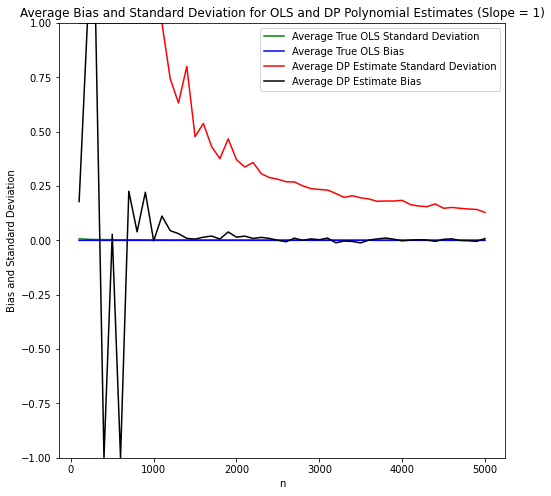
\includegraphics[width=8.0cm]{plots/Polynomial_1.png}}
\label{fig}
\end{figure}
\begin{figure}[htbp]
\centerline{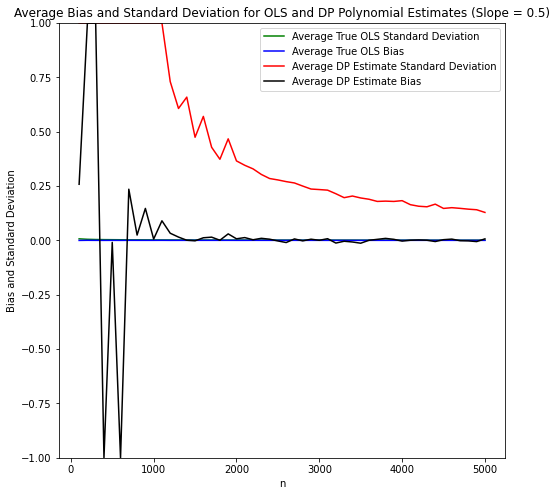
\includegraphics[width=8.0cm]{plots/Polynomial_0.5.png}}
\label{fig}
\end{figure}
\begin{figure}[htbp]
\centerline{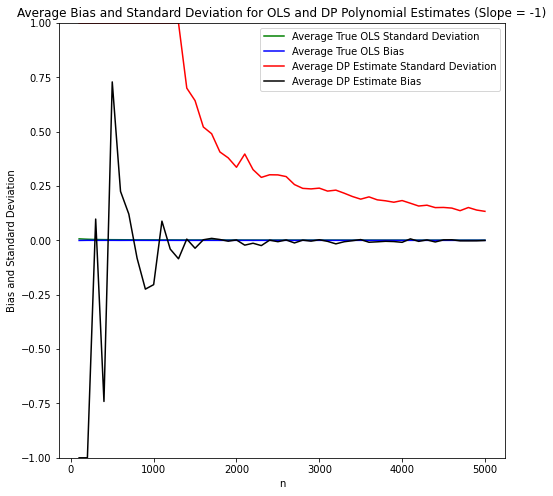
\includegraphics[width=8.0cm]{plots/Polynomial_-1.png}}
\label{fig}
\end{figure}
\newpage

\subsection{Experimental Results}
\textcolor{brown}{Looking closely, these plots show similar trends to the generated to OLS in problem set 4, but have  considerable more stable standard deviation trends. We can explain this with a number of different ways, but its likely that the added polynomial terms in polynomial regression allowed for a more nuanced fit to the data, leading to a lower standard deviation for our estimates. It's worth pointing out, however, that polynomial regressions is more susceptible to outliers, and the decrease in standard deviation comes with the possibility of a model that overfits to used data. To better see how polynomial regression can produce more legitimate results, it might be worth generalizing the data into more than one dimension, and expanding the range of values in our dataset but we expect this method to scale poorly, due to the effect of outliers on this model. We will soon explore how we can address over-fitting with more complicated regression techniques in the following sections.} 

\section{Ridge Regression}
\textcolor{brown}{Two of the methods we discuss below, ridge and lasso regression, can be characterized by a different objective function as compared to that of OLS, due to the addition of a penalty term that penalizes large values of $\theta$, and therefore encouraging regularization. The only difference between the two methods is the penalty term itself. In ridge regression, we add a penalty proportional to the $\ell_2$ norm of $\theta$, whereas in lasso regression the penalty is proportional to the $\ell_1$ norm. These penalty terms are favored in traditional machine learning literature, as they can reduce error bounds on estimators, and defend against complex estimators overfit to the data. (We remark that estimates $\theta$ with large parameter values overfit to the specific data may also be sensitive to individual perturbations in data points, posing a privacy risk; by penalizing such cases, regularization also brings a privacy benefit.) However, the differing nature of the two penalty terms in ridge and lasso regression necessitates using different approaches for creating DP versions of the techniques. As one example, Chaudhuri, Monteleoni, and Sarwate's method for empirical risk minimization applies only when the term is differentiable, which is not the case for the $\ell_1$ norm in lasso regression. The next sections are thus devoted to exploring specific DP algorithms in these two settings.}

\textcolor{brown}{}

\subsection{Discussion}
Another regression technique that should be taken into account when performing DP techniques is ridge regression [14]. When creating models to fit to data, ridge regression has proven especially useful in machine learning by penalizing model coefficients that are relatively large in magnitude, ensuring that models aren't over fit to the training data that they're given [14]. 

Here, we interpret ridge regression similarly to how OLS is interpreted earlier, with the data again modeled as $y= \theta^T X+e$. The result leads to a very similar estimator to that of the OLS objective - $\hat{\theta}_{Ridge} = (X^T X + kI_p)^{-1}X^T y$, with $k > 0$ being small and $I_p$ being the $p \times p$ identity matrix [14]. 

\subsection{Experimental Results}
Here, we will work on modifying OLS regression techniques in DP to incorporate the extra penalizing term seen in ridge regression. For this, we will be using the dataset provided for HW 4, and restrict $X$ to $N$ uniformly-generated points in the interval $[-1,1]$. Like in the OLS case, we will generate $y$ according the equation $y=X+e$, where $e\sim \Normal(0,\sigma^2)$. evaluate algorithm performance with variations in this data, we vary $N$ and $\sigma^2$ Instead of using standard OLS, however, we will insert the $kI_p$ to minimize our objective function. Below, we have included three different DP mechanism tests compared to true OLS, for three different slopes: 1, 0.5, and -1. 

\begin{figure}[htbp]
\centerline{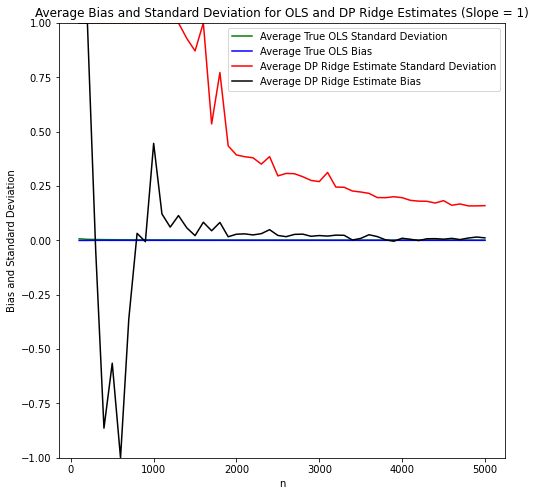
\includegraphics[width=8.0cm]{plots/ridge_1.png}}
\caption{Bias and Standard Deviation of Ridge parameter estimates for true slope $1$}
\label{fig}
\end{figure}
\begin{figure}[htbp]
\centerline{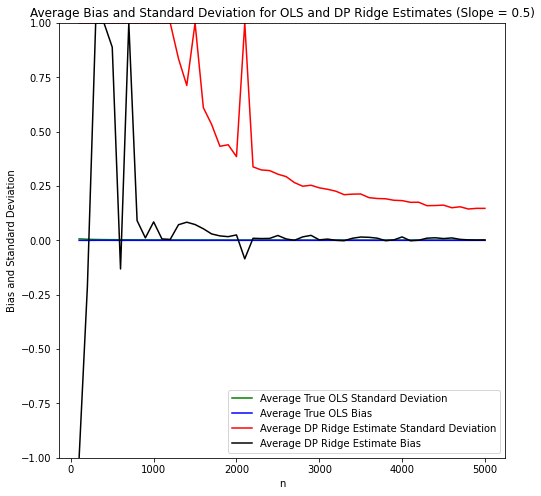
\includegraphics[width=8.0cm]{plots/ridge_0.5.png}}
\caption{Bias and Standard Deviation of Ridge parameter estimates for true slope $0.5$}
\label{fig}
\end{figure}
\begin{figure}[htbp]
\centerline{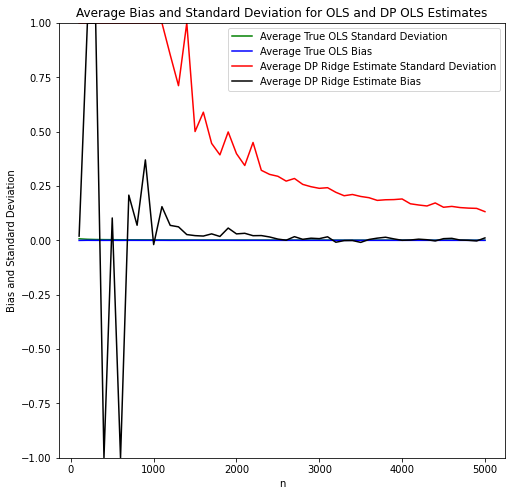
\includegraphics[width=8.0cm]{plots/ridge_-1.png}}
\caption{Bias and Standard Deviation of Lasso parameter estimates for true slope $-1$}
\label{fig}
\end{figure}

\newpage
\textcolor{brown}{Interestingly, these plots show little to no difference from the ones generated in problem set 4, when using standard OLS. There are a number of different possibilities on why this could have happened, but the most obvious one is that our generated dataset values are too restricted in range and the magnitude of the values used are too small for the correcting penalizing term of ridge regression to come into play. Making the penalizing term too large, however, completely overpowered the more subtle regression being performed by the other terms in our model. To better see how ridge regression can produce more legitimate results, it might be worth generalizing the data into more than one dimension, and expanding the range of values in our dataset.}

\section{Lasso Regression}
\subsection{Discussion}
This section focuses on discussing and implementing the ideas presented by Talwar, Thakurta, and Zhang (2015). Lasso uses the same setup and loss function as OLS, modelling $y=\theta^T X+e$ and aiming to minimize $\loss(\theta, D)=\frac{1}{n}\sum_{i=1}^n (\theta^T x_i-y_i)^2$. However, there is the additional constraint that $\|\theta\|_1\leq 1$. Lasso tends to be most applied in high-dimensional settings where $p>n$, as the constraint on $\theta$ encourages sparse parameters. (Nonetheless, implementation-wise we test the performance of this algorithm on 1D data for consistency.)

The authors give a $(\epsilon,\delta)$-DP algorithm for providing an estimate $\hat{\theta}$ based on the Frank-Wolfe algorithm. Briefly, the algorithm updates the estimate $\hat{\theta}$ in incremental steps, and assumes several technical conditions. It requires the data to be bounded in $\ell_1$---specifically by $1$. It also requires the set of all possible parameters under consideration $\theta$ to be bounded by a convex polytope, in this case the $\ell_1$-ball in $\mathbb{R}^d$, and also requires the loss function to be $\ell_1$-Lipschitz with constant $L_1$. In each step, the loss of each vertex of the polytope is computed, where Laplace noise is added for privacy. $\hat{\theta}$ is then updated in the direction of the vertex with the smallest (noisy) loss, where the magnitude of the step size decreases over time. 

Under these conditions, the authors showed that in addition to DP, the risk (Definition 5) of the algorithm is close to optimal. In particular, they show that the risk of the algorithm is of order $\frac{\log(np)\sqrt{\log(1/\delta)}}{(n\epsilon)^{2/3}}$, and any $(\epsilon, \delta)$-DP linear regression problem under the technical conditions above must have risk being $\Omega(1/(n\log n)^{2/3})$. 

% still need to figure out lipschitz
% maybe provide the algorithm
% https://math.stackexchange.com/questions/2802412/is-the-least-squares-system-lipschitz

\subsection{Experimental Results}
\textcolor{brown}{We notice that in the simple dataset example discussed in section I.C, all technical conditions are fulfilled. As we work in the one-dimensional case, the constraint on the possible set of $\theta$ being the $\ell_1$ ball reduces to only considering values of $\theta$ in $[-1, 1]$. Hence the only vertices which need to be considered in each update step in the Frank-Wolfe algorithm are the two points $-1$, $1$. By construction, all values $x_i$ and $y_i$ are also bounded in magnitude by $1$. It can also be shown that the $\ell_1$-Lipschitz constant for squared loss under these data bounds is bounded: Wang (2018) provides the fact that if our data is bounded, an appropriate Lipschitz constant for the squared loss is $L_1=\|x^*\|^2\|\theta\|+\|x^*\|\|y^*\|$ (using the $\ell_2$ norm), where $x^*$ and $y^*$ are the elements with the largest $\ell_2$ norm among $X$ and $y$. Given the data, this constant can be calculated and inputted as a parameter into the DP algorithm.}

It was thus possible to implement the algorithm on the simple dataset example, where in the Frank-Wolfe algorithm $T=100$ update steps are performed, starting with an initial estimate of $\hat{\theta}=0$. We fixed $\sigma^2=0.02$ and considered increments of $N$ from $1000$ to $5000$ in steps of $100$. In the manner of what was done in the class assignment, for each value of $N$, $100$ trials were performed. \textcolor{brown}{In each trial, the OLS and DP Lasso standard deviation and bias were calculated (recalling that the slope from the data-generating process was set to be $1$), with the results displayed below. Note that given the one-dimensional data and possible slope bounds, the Lipschitz constant for squared loss can be set to $1^2\cdot 1 + 1\cdot 1=2$. In this following plot, we also include the bias and standard deviation for the non-private lasso estimate as a point of comparison. The non-private lasso estimate is based on using the Frank-Wolfe algorithm with the same parameter bounds of $[-1, 1]$, but without adding random noise.}

\begin{figure}[htbp]
\centerline{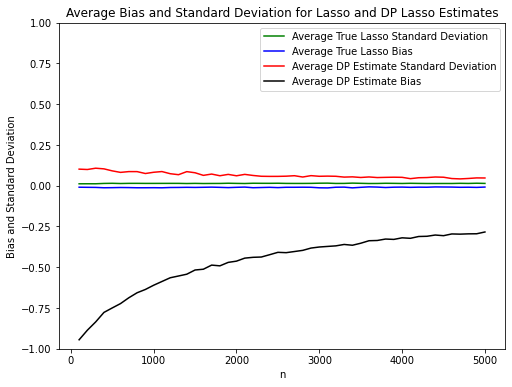
\includegraphics[width=8.5cm]{plots/lasso_1.png}}
\caption{Bias and Standard Deviation of Lasso parameter estimates for true slope $1$}
\label{fig}
\end{figure}

There are two main conclusions to be drawn from the performance of the DP technique in the plot. The first is that the variance of Lasso estimates decreases as the number of data points increases, which may hint at convergence of the Lasso estimator under this DP technique. The main conclusion of note, however, is that the bias is consistently negative (i.e. values of $\hat{\theta}$ are below $1$), but decreases in magnitude as $N$ increases. Looking at the setup of the dataset and the technical constraints, this should be no surprise. Although the data-generating process used a slope of $1$, the DP formulation considers only possible $\theta$ in the range $[-1,1]$, with one of the vertices used to perform updates being $1$. In other words, the true $\theta$ is on the boundary of our possible parameter space, which explains the consistent bias. \textcolor{brown}{We note, however, that the ordinary, non-private lasso technique works very well in estimating the slope, with low variance and bias, despite this fact. It appears that the difficulty in determining an estimate on the border of the parameter space arises not because of the Frank-Wolfe algorithm, but because the added noise for DP makes it hard for the estimate to consistently take update steps in the right direction.} 

\textcolor{brown}{Indeed, as further illustrative examples, we find a similar positive bias when our true slope is set to $-1$, and we find a significant decrease in the bias when our true slope is set to be $0.5$, which lies within the parameter range, as shown below. Finally, when the true slope is set to be $0$, which equals the initial value of our estimator, the bias stays near $0$ throughout. This demonstrates that the bias of the slope estimate is significantly influenced by the required bounds on the space of possible slopes. Results are shown in Figures 5-7.}

\begin{figure}[htbp]
\centerline{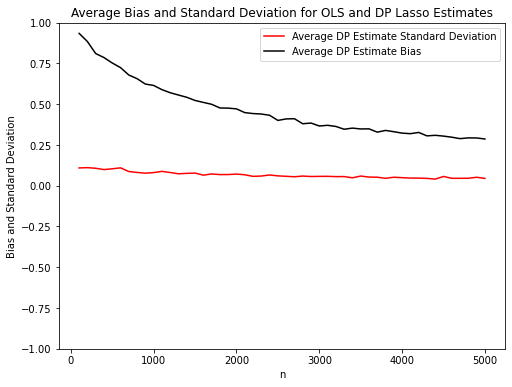
\includegraphics[width=8.5cm]{plots/lasso_-1.png}}
\caption{Bias and Standard Deviation of Lasso parameter estimates on $n$ data points for true slope $-1$} \bigskip
\centerline{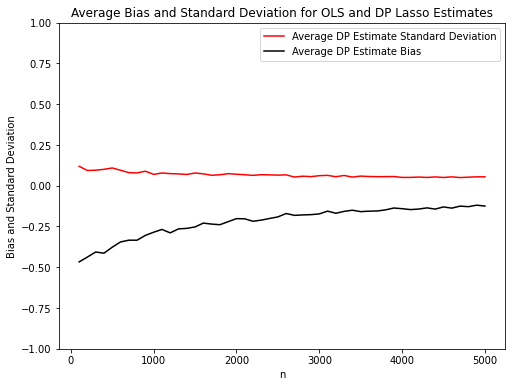
\includegraphics[width=8.5cm]{plots/lasso_0.5.png}}
\caption{Bias and Standard Deviation of Lasso parameter estimates on $n$ data points for true slope $0.5$}
\centerline{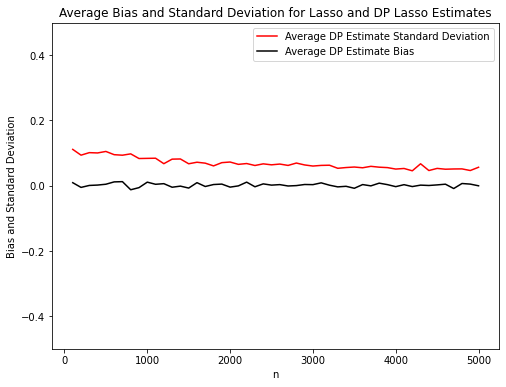
\includegraphics[width=8.5cm]{plots/lasso_0.png}}
\caption{Bias and Standard Deviation of Lasso parameter estimates on $n$ data points for true slope $0$}
\label{fig}
\end{figure}

\textcolor{brown}{To evaluate the performance of DP lasso regression on variants of this dataset, we also consider fixing the number of data points at $2000$, the true slope at $c=0.5$, $\epsilon=1$, and $\delta=1\cdot 10^{05}$, while varying $\sigma^2$ from $0.02$ to $0.5$ in increments of $0.01$, again recording the bias and standard deviation of the estimated slopes over $100$ trials. In another setting, we do the same with $\sigma^2$ fixed at $0.1$, we vary $\epsilon$ from $0.1$ to $10$, with $50$ points logarithmically spaced. These produce the diagrams shown in figures 8 and 9. Modifying $\sigma^2$ does not seem to produce a large impact on the bias or standard deviation, suggesting that the DP Lasso regression method can perform well even when a linear trend is not obvious. As expected, the bias and standard deviation decrease with increasing $\epsilon$, as an increasing privacy budget decreases the required noise added to each step of the algorithm, producing more accurate results.}

\begin{figure}[htbp]
\centerline{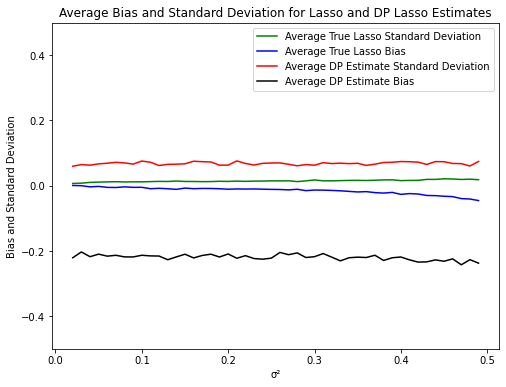
\includegraphics[width=8.5cm]{plots/lasso_sigmas.png}}
\caption{Bias and Standard Deviation of Lasso parameter estimates with standard deviation $\sigma^2$ for true slope $0.5$} \bigskip
\centerline{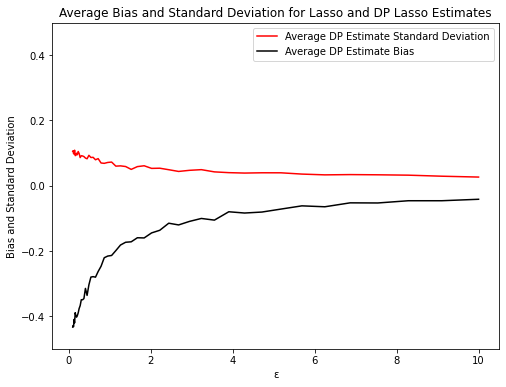
\includegraphics[width=8.5cm]{plots/lasso_epsilon.png}}
\caption{Bias and Standard Deviation of Lasso parameter estimates with epsilon privacy parameter $\epsilon$ for true slope $0.5$}
\label{fig}
\end{figure}

\section{Bayesian Linear Regression}
We note that all the linear regression techniques up to this point have been frequentist, producing point estimates of $\theta$. However, there has also been work in the literature which focuses on analyzing Bayesian inference techniques in a DP manner as well, which forms the focus of this section. The techniques implemented are drawn from the work of Bernstein and Sheldon (2019).

\subsection{Discussion} Unlike the settings above, in Bayesian linear regression the response data are modeled to follow a conditional Normal (Gaussian) distribution, instead of adding error terms: $y|\theta, \sigma^2\sim \Normal(\theta^T X, \sigma^2)$. In the authors' setting, we assume that both $\theta$ and $\sigma^2$ are unknown, with the canonical conjugate priors $\sigma^2\sim \textrm{InvGamma}(a_0,b_0)$ and $\theta|\sigma^2\sim \Normal(\mu_0,\sigma^2\Lambda_0^{-1})$, where $a_0,b_0$ are constants, $\mu_0$ is a $d$-dimensional vector of means, and $\Lambda_0$ is the prior $d\times d$ invertible covariance matrix. Alternatively, $(\theta, \sigma^2)$ follow a Normal-Inverse Gamma distribution, $NIG(\mu_0,\Lambda_0,a_0,b_0)$. By conjugacy it is known that the posterior is also Normal-Inverse Gamma, i.e. $p(\theta, \sigma^2|X,y)\sim NIG(\mu_n,\Lambda_n,a_n,b_n)$, where the parameters are updated as follows: 
\begin{align*}
    \mu_n &= (X^T X+\Lambda_0)^{-1}(X^T y+\mu_0^T \Lambda_0) \\
    \Lambda_n &= X^T X+\Lambda_0 \\
    a_n &= a_0+n/2 \\
    b_n &= b_0+\frac{1}{2}(y^T y+\mu_0^T \Lambda_0 \mu_0-\mu_n^T\Lambda_n\mu_n)
\end{align*}

When both these quantities are unknown, in addition to $X^T X$ and $X^T y$ we need a third sufficient statistic $y^T y$. In our case, we will also address the case where $\sigma^2$ is fixed and known in advance, and therefore only the prior and posterior distributions of $\theta$ need to be dealt with. In this case, only the two sufficient statistics $X^T X$ and $X^T y$ are needed. Then the posterior update is simplified noticeably to $p(\theta|X,y)\sim \Normal((X^T X+\Lambda_0)(X^T y+\mu_0^T\Lambda_0), X^T X+\Lambda_0)$. Furthermore, when all data is one-dimensional, each of the elements in the formula for the posterior reduce to scalars. 

Bernstein and Sheldon discuss that a sufficient way to implement Bayesian linear regression in an $\epsilon$-DP manner is to perturb the sufficient statistics with noise via the Laplace mechanism. Defining $\Delta_{X^T X}$, $\Delta_{X^T y}$, and $\Delta_{y^T y}$ as the maximum variation of those statistics adjusting for dimensionality, for each statistic $s$ random noise of $\textrm{Lap}(\Delta_{s_i}/\epsilon)$ is added. Let these original nad noisy sufficient statistics be written as $s$ and $z$ respectively. Given these statistics, the authors then propose three methods to effectively use Bayesian linear regression using these sufficient statistics. The first simply treats the sufficient statistics as if they were the true statistics, thus comprising a ``noise-naive'' method for reporting the posterior update. While the authors show that this method produces an asymptotically correct posterior and we investigate this method in our experiments, they also propose two more nuanced methods.

Both of these methods are noise-aware, incorporating the existence of noise into the model: conditioning on the data $X$ can no longer be assumed. The first method assumes that a prior has been specified, $p(X)$, and models the posterior as $p(\theta, \sigma^2|z)\propto \int p(X)p(\theta, \sigma^2)p(y|X,\theta, \sigma^2)p(z|X,y)p\, dX\, dy$, using MCMC sampling to approximate the distribution. The second method performs inference directly over $s$, based on the fact $p(\theta, \sigma^2|z)\propto \int_s p(\theta, \sigma^2,s,z)\, ds$. A Gibbs sampler can be developed to draw from the conditional distributions, $p(\theta, \sigma^2)$ and $p(s|\theta, \sigma^2, z)\propto p(s|\theta, \sigma^2)p(z|s)$. Although these methods are more technically sophisticated and far less simple, the authors demonstrate that it quantifies posterior uncertainty far better.

\subsection{Experimental Results}
Again we use the simple dataset scheme described in section I.C (with the slope therefore being $1$). We set $\sigma^2=0.5$, and generate four datasets, varying values of $N\in\{10,20,50,100\}$. The priors for the mean and variance on the slope are $0$ and $1$, respectively. In the plots displayed below, each dataset is displayed as a scatter plot with the Bayesian linear regression approximations overlaid. The line representing the slope calculated using the raw data is displayed in blue, while the line representing the slope calculated using the ``noise-naive'' DP method is displayed in red. Shaded regions indicate plots for the $95\%$ confidence intervals given the posterior variance for the slope values (i.e. the upper bound of the shaded region denotes the smallest slope value in the confidence interval, and similarly for the lower bound). \textcolor{brown}{Due to $y$ values being clipped, the most accurate slope estimate for the data may not be $1$. Instead, we include the non-private OLS slope estimate on the plot as a point of comparison.}

A few quick qualitative observations can be made. First, the width of the $95\%$ confidence intervals in slope space decreases with $N$, which is unsurprising as we observe more data and the posterior variance decreases. However, as can be throughout the figures, the noise added to small values of the posterior variance can result in slope ranges which do not capture the true slope of the data-generating process. \textcolor{brown}{Second, the overall accuracy of the DP estimate approximates the raw estimate as $N$ increases; this is likely due to larger magnitudes of the sufficient statistics having a greater influence on the posterior values, with the magnitude of the overall noise being added becoming less significant. Indeed, in the $N=500$ case, we find that the OLS estimate, Bayes estimate, and DP Bayes estimate are nearly identical, narrowing down to point estimates.}

\begin{figure}[htbp]
\centerline{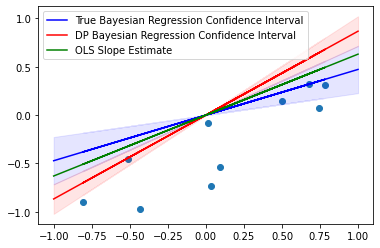
\includegraphics[width=8cm]{plots/bayes_10.png}}
\caption{Raw and DP posterior estimates for $N=10$} \bigskip
\centerline{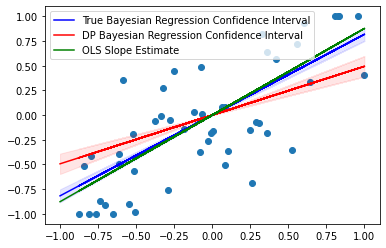
\includegraphics[width=8cm]{plots/bayes_50.png}}
\caption{Raw and DP posterior estimates for $N=50$} \bigskip
\centerline{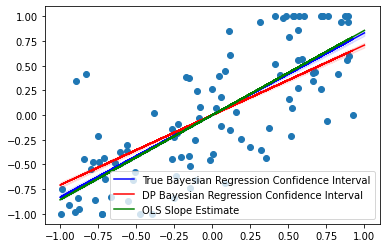
\includegraphics[width=8cm]{plots/bayes_100.png}}
\caption{Raw and DP posterior estimates for $N=100$} \bigskip
\centerline{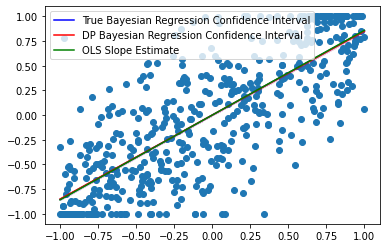
\includegraphics[width=8cm]{plots/bayes_500.png}}
\caption{Raw and DP posterior estimates for $N=500$} \bigskip
\label{fig}
\end{figure}

\textcolor{brown}{There are, however, pitfalls to this method, especially when $N$ is small. Note that in Figures 11 and 12, the 95\% confidence interval of the slope excludes the true slope of $1$. We also encountered runs in which the approximations were much less accurate, due to the magnitude of the Laplacian noise obfuscating the actual posterior values. In cases like these, the overall result of the linear regression is worthless, similar to other situations discussed in class. For instance, in Figure 14 below there is an example of such a ``bad'' run. This may highlight the need for more sophisticated techniques such as the one developed by the authors.}

\begin{figure}[htbp]
\centerline{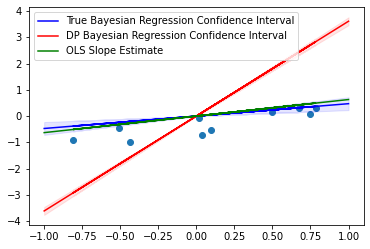
\includegraphics[width=8cm]{plots/bayes_bad.png}}
\caption{Another trial featuring raw and DP posterior estimates for $N=10$} 
\label{fig}
\end{figure}

\textcolor{brown}{To quantify the overall reliability of the DP Bayes technique, we can follow a similar approach to how Lasso estimates were evaluated: treating the DP posterior mean as a point estimate, in each setting we take $100$ trials and calculate the means' variance and bias over the trials as compared to the OLS estimate. As a point of comparison, we also do the same for the non-private Bayes mean estimate, plotting both results. As standard settings, we keep the same data bounds of $[-1, 1]$ and generating slope of $1$, and fix $\epsilon=1$, $\sigma^2=0.5$, $N=500$. In the first plot we vary $N$ from $50$ to $1000$ in increments of $10$; in the second we vary $\sigma^2$ from $0.05$ to $0.75$ in increments of $0.01$; and in the last we vary $\epsilon$ from $0.1$ to $10$ in the same spacing as used for lasso regression. The results are shown in the plots below.}

\textcolor{brown}{Under our current parameter settings, we find that we need a substantially large number of data points (according to Figure 15, more than $250$) in order to have our bias and variance for the DP Bayes estimates behave consistently. As our data gets noisier with increasing $\sigma^2$, our overall DP variance and bias do not change in behavior, suggesting that the main source of noise under these parameters is still the noise added in the DP algorithm (compare this with increasing trend in the variance of non-private Bayes estimates). Finally, we also notice that for small $\epsilon<1$, the DP estimates also exhibit high variance and unpredictable values of bias. Overall, we find that this basic DP implementation tends to be particularly ill-behaved when in situations with less data or less of a privacy budget.}

\begin{figure}[htbp]
\centerline{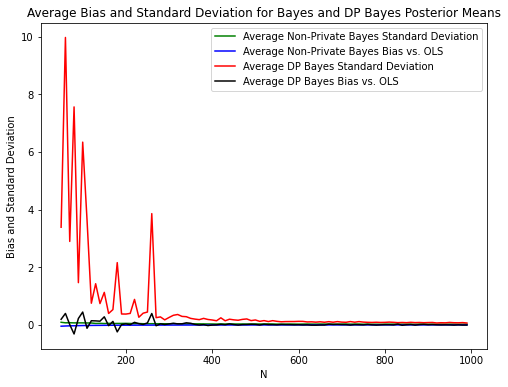
\includegraphics[width=8cm]{plots/bayes_N.png}}
\caption{Non-Private and DP Bayes posterior mean estimate variance and bias for varying $N$} \bigskip
\centerline{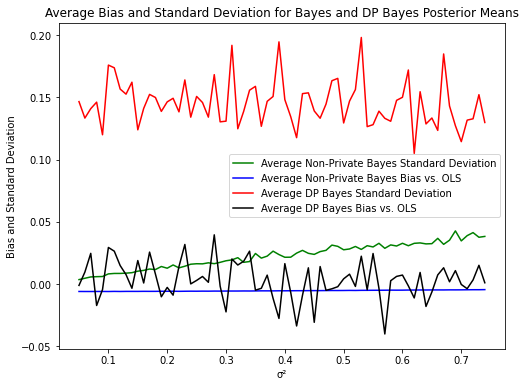
\includegraphics[width=8cm]{plots/bayes_variance.png}}
\caption{Non-Private and DP Bayes posterior mean estimate variance and bias for varying $\sigma^2$} \bigskip
\centerline{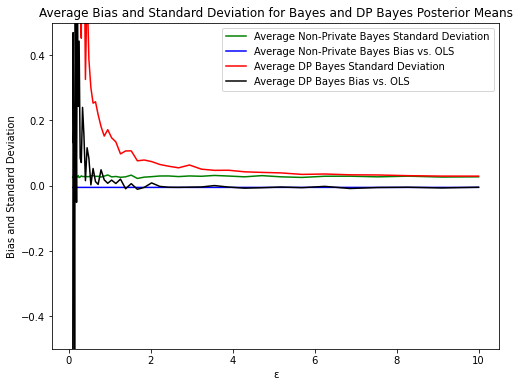
\includegraphics[width=8cm]{plots/bayes_epsilon_zoom.png}}
\caption{Non-Private and DP Bayes posterior mean estimate variance and bias for varying $\epsilon$ (with $y$-axis range limited; for small $\epsilon$, variance values exceeded $10$)} \bigskip
\label{fig}
\end{figure}

\section{Conclusion}
\color{brown}
Having presented our results from the experimental implementations above, we can now draw compare and contrast some of the conclusions we found across regression techniques. The bias and standard deviation trends for slope parameters determined through DP polynomial regression indicates that we can achieve stable estimates given a moderate number $\sim 1000$ data points, exhibiting the same, if not, improved behavior as compared to the trends found in teh course problem set. Notice that structurally, DP polynomial regression can also handle a wide range of different, non-linear data, making it broadly applicable. However, the fact that it is more sensitive to outliers could make it ill-fit in situations with noisy data.

Ridge and lasso regression both avoid overfit through regularization. Our experiments with lasso regression is similar in that it emulates the same stability as polynomial regression. Our experiments with ridge regression, however, does not possess the same stability as lasso, resulting in a similar plot to our OLS tests from problem set 4. We also found that the lasso algorithm performed well even as the data became more noisy. From these preliminary results, it might seem that for point estimates, lasso is preferred. However, it is worth noting that lasso regression was implemented under many technical restrictions, such as determining a fixed space of possible solutions for the slope estimate \textit{a priori}, and calculating a Lipschitz constant for the squared loss (which may increase substantially when outside the data bound of $[-1, 1]$, therefore increasing the noise added in the DP algorithm). Ridge regression seems better-suited for general situations where we cannot make these technical assumptions due to a lack of information.

The paradigm behind using Bayesian linear regression is different entirely, based on confidence intervals rather than point estimates. However, as we saw in the experimentation above, using a naive noise-blind DP implementation can also lead to confidence intervals that do not capture the true value, especially when we have less data points or a smaller privacy budget. Nevertheless, the low variance and bias among posterior slope estimates in settings where we can set higher $\epsilon$ or have more than a few hundred data points means that this approach may be useful and fairly similar to the non-private Bayesian regression approach in those cases.

There a lot of natural next steps for this survey. As mentioned in some earlier sections, the generated dataset for these experiments is very limited in nature. We relegate all our data to a simple interval, $[-1, 1]$, and only add Gaussian noise. The conclusions we draw from the techniques above are thus based on very limited evidence, and only consistute a first look at an implementation. As mentioned in some of the earlier sections, It is worth exploring how these techniques would fare when using a multi-dimensional dataset. One of the simplest possible ways to introduce this would be to introduce another input variable, $x_2$ that is randomly chosen from a uniform distribution and see if regressions techniques such as lasso and ridge regression can tell that $x_2$ plays no role when determining the output $y$, and that the output depends entirely on our original generated inputs.

% bayes mean variance, bias
% bayes in conclusion
% troubling confidnece intervals, from noisy suff stats

\color{black}

\begin{thebibliography}{00}
\bibitem{b1} Alabi, D., McMillan, A., Sarathy, J., Smith, A., Vadhan, S. (2020). Differentially Private Simple Linear Regression. https://arxiv.org/pdf/2007.05157.pdf. 
\bibitem{b2} Covington, C., He, X., Honaker, J., Kamath, G. (2021). Unbiased Statistical Estimation and Valid
Confidence Intervals Under Differential Privacy. https://arxiv.org/pdf/2110.14465.pdf. 
\bibitem{b3} Wang, Y.-X. (2018). Revisiting differentially private linear regression: optimal and adaptive prediction \& estimation in unbounded domain. https://arxiv.org/pdf/1803.02596.pdf. 
\bibitem{b4} Piazza, T. (2021). Differentially Private Ridge Regression. https://privacytools.seas.harvard.edu/files/privacytools/files/\-differentially\_private\_ridge\_regression.pdf.
\bibitem{b5} Talwar, K., Thakurta, A., Zhang, L. (2015). Nearly-Optimal Private LASSO. https://papers.nips.cc/paper/2015/file/ 52d080a3e172c33fd6886a37e7288491-Paper.pdf. 
\bibitem{b6} Bernstein, G., Sheldon, D. (2019). Differentially Private Bayesian Linear Regression. https://arxiv.org/pdf/1910.13153.pdf. 
\bibitem{b7} Bernstein, G. (2019). private\_bayesian\_regression. Github repository. https://github.com/gbernstein6/private\_bayesian\_ regression.
\bibitem{b8} Chetty, R., Friedman, J. (2019). A practical method to reduce privacy loss when disclosing statistics based on small samples. https://opportunityinsights.org/wp-content/uploads/2019/03/w25626.pdf. 
\bibitem{b9} Chaudhuri, K., Monteleoni, C. (2008). Privacy-preserving logistic regression. https://papers.nips.cc/paper/2008/file/ 8065d07da4a77621450aa84fee5656d9-Paper.pdf. 
\bibitem{b10} Yu, F., Rybar, M., Uhler, C., Fienberg, S. (2014). Differentially-Private Logistic Regression for
Detecting Multiple-SNP Association in GWAS
Databases. https://arxiv.org/pdf/1407.8067.pdf 
\bibitem{b11} Dwork, C., Roth, A. (2014). The Algorithmic Foundations of Differential Privacy. https://www.cis.upenn.edu/
\~aaroth/Papers/privacybook.pdf. 
\bibitem{b12} Chetty, R., Friedman, J. (2019). A Practical Method to Reduce Privacy Loss when Disclosing Statistics Based on Small Samples. https://opportunityinsights.org/paper/differential-privacy/. 
\bibitem{b13} Chaudhuri, K., Monteleoni, C., Sarwate, A. D. (2011). Differentially Private Empirical Risk Minimization. https://jmlr.org/papers/volume12/chaudhuri11a/chaudhuri11a.pdf. 
\bibitem{b14} Hoerl, A., Kennard, R. (1970). Ridge Regression: Biased Estimation for Nonorthogonal Problems.
\bibitem{b15} Ostertagová, H. (2012). Modelling using Polynomial Regression
\end{thebibliography}
\end{document}
